\section{Пример 1: результаты тестов}
В таблице 7.1 показаны данные результатов тестов из Mardia, Kent and Bibby (1979); $n = 88$ студентов сдавали пять тестов: по механике, векторному исчислению, алгебре, математическому анализу, и статистике.

На первых двух тестах не разрешалось использовать учебник, на остальных учебник был разрешён. Удобно представлять эти данные как матрица  данных $\mathbf X$ размерности $88 \times 5$, где $i$-ая строка есть
\begin{equation}
	\mathbf x_i = (x_{i1}, x_{i2}, x_{i3}, x_{i4}, x_{i5})
\end{equation}
--- пять результатов $i$-го студента, $i = 1,2,\ldots,88.$

Вектор средних $\bar{\mathbf{x}} = \sum_{i = 1}^{88} \mathbf{x}_i/88$ есть вектор средних по столбцам:
\begin{equation}
	\bar{\mathbf x} = (38.95, 50.59, 50.60, 46.68, 42.31).
\end{equation}
 Эмпирическая ковариационная матрица $\mathbf G$ --- это матрица $5 \times 5$, где $(j, k)$-й элемент равен
 
\begin{equation}
G_{jk} = \frac{1}{88}\sum_{i = 1}^{88} (x_{ij} - \bar x_j) (x_{ik} - \bar x_k) \qquad j,k = 1,2,3,4,5.
\end{equation}

Заметим, что диагональные элементы $G_{jk}$ это оценки дисперсии результатов теста $j$ методом подстановки. Получим матрицу
\newline
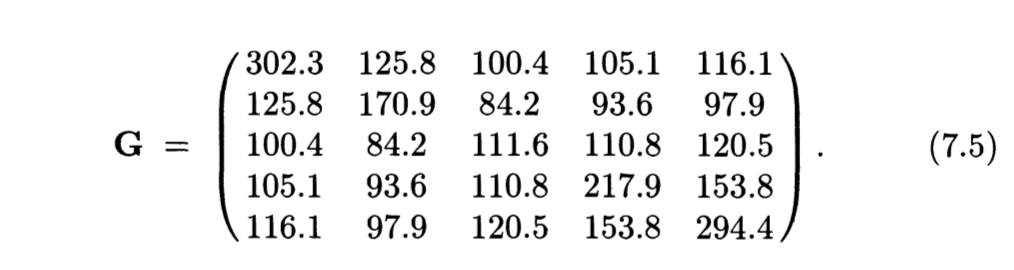
\includegraphics[width=0.85\linewidth]{6/e75.png}
\newline

\setcounter{equation}{5}
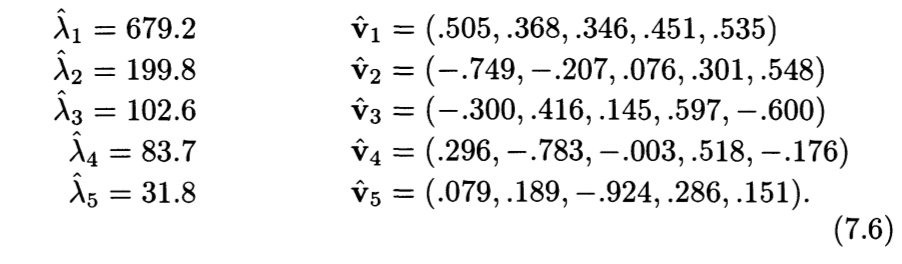
\includegraphics[width=0.85\linewidth]{6/e76.png}
\newline

\setcounter{equation}{6}
Какой интерес представляют собственные значения и векторы ковариационной матрицы? Они помогают описать структуру высокоразмерных данных (как в случае с таблицей (7.1)) в которых описано большое число независимых величин ($n = 88$ студентов), но при этом имеются коррелированные измерения для каждого студента. Заметьте, что пять тестовых оценок высоко коррелированы. Студент, который хорошо сдал тест по механике, вероятно также хорошо сдал тест и по векторам и т.д. Очень простая модель для коррелированных оценок имеет вид
\begin{equation}
	\mathbf x_i = Q_i \mathbf v, \qquad i = 1,2,\ldots,88.
\end{equation}

\noindent
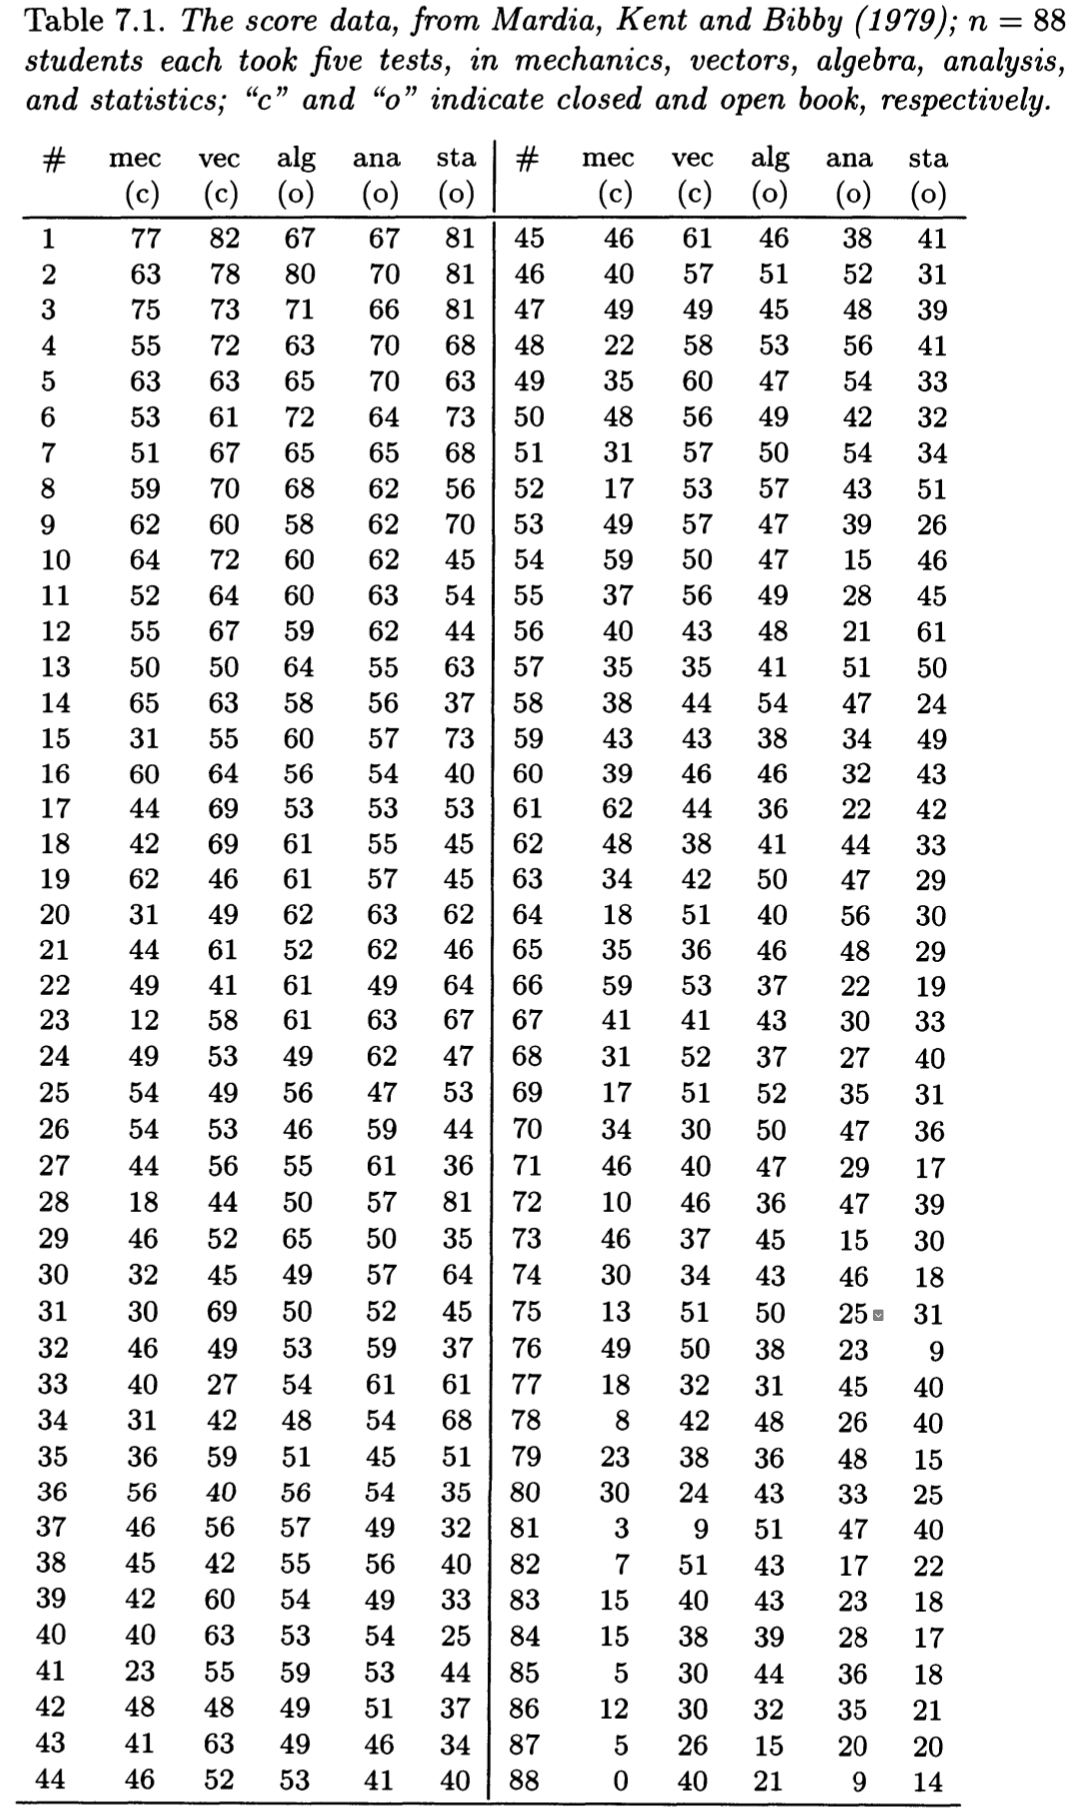
\includegraphics[width=0.9\linewidth]{6/t71.png}
\newline
\setcounter{table}{1}

$Q_i$ является числом, представляющим способности $i$-го студента, в то время как $\mathbf v = (v_1,v_2,v_3,v_4,v_5)$ есть фиксированный вектор из 5 чисел, определённый для всех студентов. $Q_i$ можно рассматривать как общую оценку интеллектуальных способностей студента $i$ (IQ). Изначально IQ были мотивированы именно моделями чуть сложнее, чем (7.7).

Если бы модель (7.7) была верна, мы бы смогли это определить из собственных значений: только $\hat \lambda_1$ было бы положительным, остальные --- $\hat \lambda_2, \hat \lambda_3, \hat \lambda_4, \hat \lambda_5$ --- равнялись бы нулю; также первый собственный вектор $\hat{\mathbf v}_1$ был бы равен $\mathbf v$. Пусть $\hat \theta$ есть частное наибольшего собственного значения и их суммы, то есть
\begin{equation}
	\hat \theta = \hat \lambda_1 / \sum_{i = 1}^5 \hat \lambda_i.
\end{equation}
Модель (7.7) эквивалентна $\hat \theta = 1$. Конечно, мы не можем ожидать, что для таких зашумлённых данных, как оценки, модель (7.7) окажется точной, даже если модель фундаментально верна.

Рисунок 7.1 даёт стилизованную иллюстрацию этого замечания. Мы взяли только две из оценок и отобразили слева ситуацию, если бы одно число $Q_i$ идеально отражало обе оценки. Оценки лежат на одной прямой; $Q_i$ можно считать как расстояние вдоль прямой до каждой точки от начала координат. Рисунок справа показывает более реалистичную ситуацию. Точки не лежат вдоль прямой, но расположены близко к ней. Прямая на графике коллинеарна направлению, заданному первым собственным вектором ковариационной матрицы. Эта прямая иногда называется \textit{прямой первой главной компоненты} и имеет следующее свойство: она минимизирует сумму квадратов расстояний между точками и прямой (в отличие от метода наименьших квадратов, который заключается в минимизации суммы квадратов вертикальных расстояний до прямой). Эти расстояния показаны на рисунке справа в виде небольших отрезков. Сложно создать такой график для всех данных об оценках: прямая главной компоненты была бы прямой в пятимерном пространстве, лежащей ближе всего к данным. Если рассмотреть проекцию каждой из точек на прямую, прямая первой главной компоненты  также будет минимизировать выборочную дисперсию всех спроецированных точек.

Для данных о тестировании студентов получим
\begin{equation}
  \hat \theta = \frac{679.2}{679.2+199.8+\ldots+31.8} = 0.619.
\end{equation}
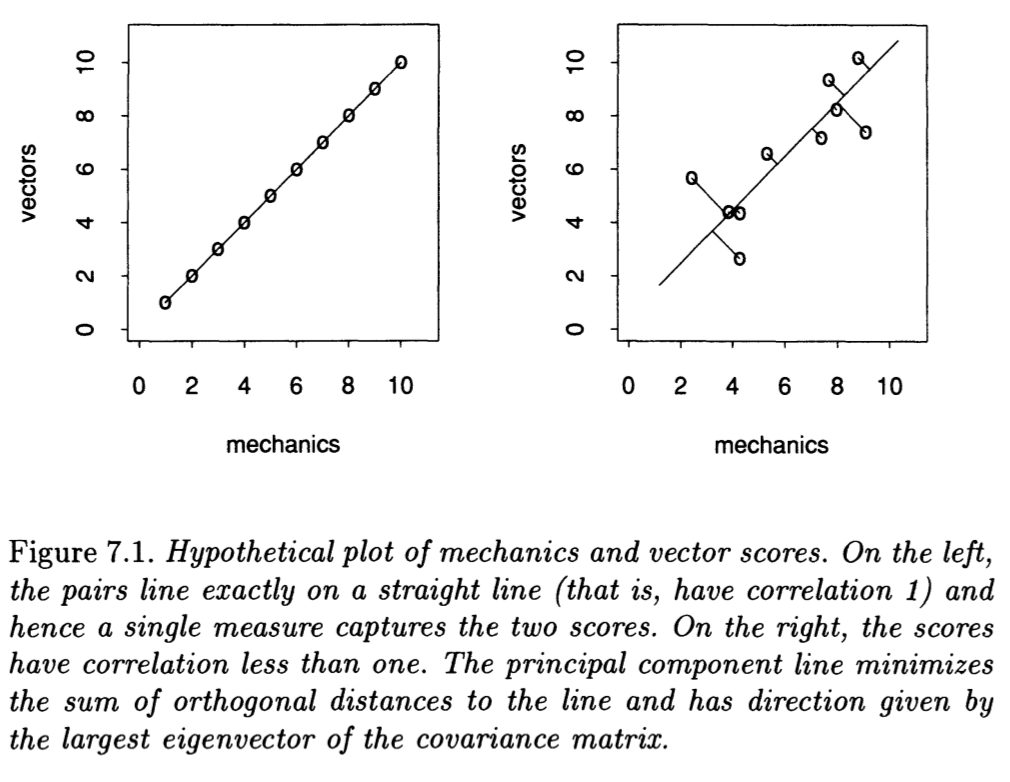
\includegraphics[width=0.85\linewidth]{6/f71.png}
\setcounter{figure}{1}

Во многих ситуациях такое большое значение $\hat \theta$ можно считать достаточно любопытным, что показывает высокую степень предсказательной силы модели (7.7).
Значение $\hat \theta$ измеряет процент дисперсии, объясняемой первой главной компонентой. Чем ближе точки лежат к прямой первой главной компоненты, тем выше значение $\hat \theta$.
Насколько точна оценка $\hat \theta$? Именно для ответа на такие вопросы бутстреп и был создан. Математическая сложность вычисления $\hat \theta$ не важна до тех пор пока мы можем подсчитать $\hat \theta^*$ для любых бутстреп данных. В этом случае бутстреп выборка представлена $\mathbf X^*$ --- матрицей $88\times 5$. Строки $\mathbf x_i^*$ матрицы $\mathbf X^*$ есть случайная выборка размера 88 из столбцов оригинальной матрицы $\mathbf X$
\begin{equation}
	\mathbf x_1^* = \mathbf x_{i_1}^*,\,\mathbf x_2^* = \mathbf x_{i_2}^*, \ldots,\, \mathbf x_{88}^* = \mathbf x_{i_{88}}^*, 
\end{equation}
как в (6.4). Некоторые строки матрицы $\mathbf X$ не появляются ни разу, некоторые один раз, некоторые дважды, и т.д., в итоге имеется 88 строк.

Сгенерировав матрицу $\mathbf X^*$, мы считаем её ковариационную матрицу $\mathbf G^*$ по аналогии с (7.4)
\begin{equation}
G_{jk}^* = \frac{1}{88}\sum_{i = 1}^{88} (x_{ij}^* - \bar x_j^*) (x_{ik}^* - \bar x_k^*), \qquad j,k = 1,2,3,4,5.
\end{equation}

Затем вычисляем собственные значения матрицы $\mathbf G^*$ --- $\hat \lambda_1^*, \hat \lambda_2^*,\ldots,\hat \lambda_5^* $ --- и в конце
\begin{equation}
	\hat \theta^* = \hat \lambda_1^* / \sum_{i = 1}^5 \hat \lambda_i^*,
\end{equation}
На рисунке 7.2 изображена гистограмма $B = 200$ репликаций бутстреп оценок $\hat \theta^*$. 
\newline
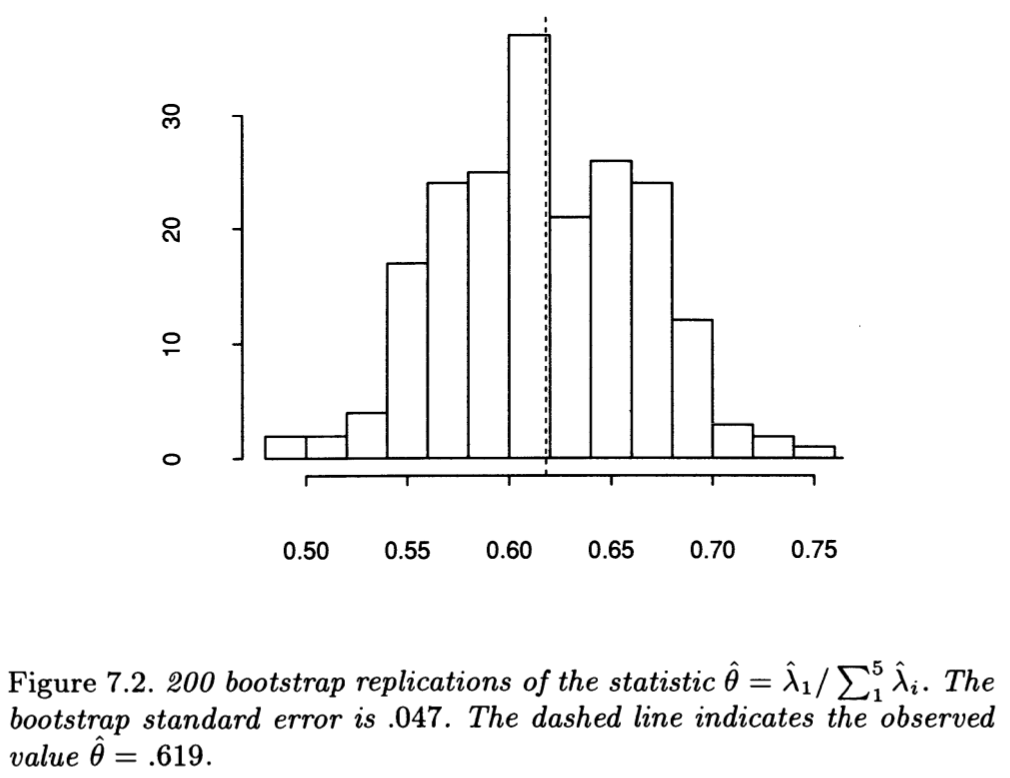
\includegraphics[width=0.85\linewidth]{6/f72.png}
\newline
\setcounter{figure}{2}

Они дают следующую оценку стандартной ошибки $\hat \theta^*$: $\widehat{\text{se}} = 0.047$. Среднее для всех 200 репликаций составило $0.625$, что лишь немногим больше, чем $\hat \theta = 0.619.$ Это означает, что $\hat \theta$ близка к несмещённой. Гистограмма выглядит адекватно, но $B = 200$ всё же недостаточно для того, чтобы ясно увидеть форму распределения. Некоторые квантили эмпирического распределения $\hat \theta^*$ показаны в таблице 7.2.

\noindent
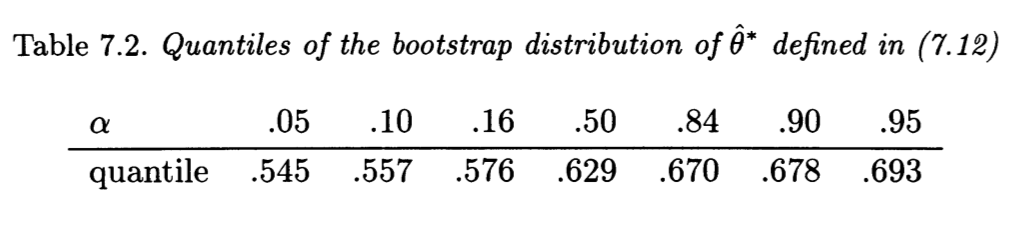
\includegraphics[width=0.9\linewidth]{6/t72.png}
\newline
\setcounter{table}{2}

\textit{Стандартный доверительный интервал} для настоящего значения $\theta$ (значениe $\hat \theta$, если устремить $n \rightarrow \infty$)
\begin{equation}
  \theta \in \hat \theta \pm z^{(1-\alpha)} \cdot \widehat{\text{se}} \qquad \text{(с вероятностью $1 - 2\alpha$)}
\end{equation}
где $z^{(1-\alpha)}$ есть $100(1- \alpha)$ персентиль стандартного нормального распределения; $z^{(.975)} = 1.960,z^{(.95)} = 1.645,z^{(.841)} = 1.000$, и т.д. Вычисление интервала основано на применении асимптотической теории, которая распространяет (5.6) на генеральные статистики $\hat \theta$. В нашем случае 
$$
\theta \in 0.619 \pm 0.047 = [ 0.572,0.666]\quad \text{с вероятностью }  0.683 
$$

$$
\theta \in 0.619 \pm 0.077 = [ 0.542,0.696]\quad \text{с вероятностью }  0.900. 
$$

В 12--14 главах обсуждаются улучшенные бутстреп доверительные интервалы, менее зависимые от асимптотической теории нормального распределения.

Случайный вектор $\hat{\mathbf v}_1$, относящийся к первому собственному значению, называется первой главной компонентой $\mathbf G$. Предположим, что мы хотим выразить результаты студента одним числом, а не пятью (например, для некоторого общего оценивания). Можно показать, что наилучшая линейная комбинация оценок есть 
\begin{equation}
  y_i = \sum_{k=1}^5 \hat{v}_{1k} x_{ik},
\end{equation}
то есть линейная комбинация, использующая компоненты $\hbv_1$ как веса. Эта линейная комбинация --- <<наилучшая>> в смысле того, что среди всех возможных $\mathbf v$ она отражает наибольшую вариативность в данных по пяти оценкам. Если же мы хотим описать успеваемость студента двумя числями, например $(y_i,z_i)$, вторая линейная комбинация должна выглядеть так

\begin{equation}
  y_i = \sum_{k=1}^5 \hat{v}_{2k} x_{ik},
\end{equation}
где веса взяты из второй главной компоненты $\hbv_2$, второго собственного значения матрицы $\mathbf G$.

Веса, заданные главными компонентами, часто дают понимание структуры многомерного набора данных. Для данных с оценками интерпретация будет следующей: первая главная компонента $$\hbv_1 = (0.51, 0.37, 0.35, 0.45, 0.54)$$ накладывает положительные веса примерно одинакового размера на каждый из тестов, то есть $y_i$ условно эквивалентно взятию суммарной (или средней) оценки $i$-го студента. Вторая главная компонента $$\hbv_2 = (-0.75, -0.2, 0.08, 0.30, 0.55)$$ даёт отрицательные веса двум тестам без использования конспекта и положительные на три теста с использованием конспекта, так что $z_i$ есть показатель \textit{разницы} оценок между тестами с открытым и закрытым конспектом для $i$-го студента. (Студент с высокой оценкой $z$ гораздо лучше справился с тестами с открытым конспектом, чем с закрытым.)

Векторы главных компонент $\hbv_1$ и $\hbv_2$ есть суммарные статистики, как и $\thetahat$, несмотря на то, что у каждой из них есть несколько компонент. Мы можем применить бутстреп анализ для того, чтобы узнать, насколько они устойчивы. Те же 200 бутстреп выборок, с помощью которых мы получили $\thetahat^*$, дают бутстреп репликации $\hbv_1^*$ и $\hbv_2^*$. Они могут быть посчитаны как первые два собственных вектора $\mathbf G^*$, (7.11).

В таблице 7.3 показаны $\seh_{200}$ для каждой из компонент векторов $\hbv_1$ и $\hbv_2$. Первое, что можно заметить --- это более высокую точность $\hbv_1$; бутстреп стандартная ошибка компонент $\hbv_1$ составляет менее половины ошибки $\hbv_2$. В таблице 7.3 также указаны основанные на персентилях робастные бутстреп стандартные ошибки $\sew_{200,\alpha}$, посчитанные для $\alpha = 0.84, 0.9, 0.95$. Для компонент $\hbv_1$ $\sew_{200, \alpha}$ примерно равно $\seh_{200}$. 
\\~\\
\noindent
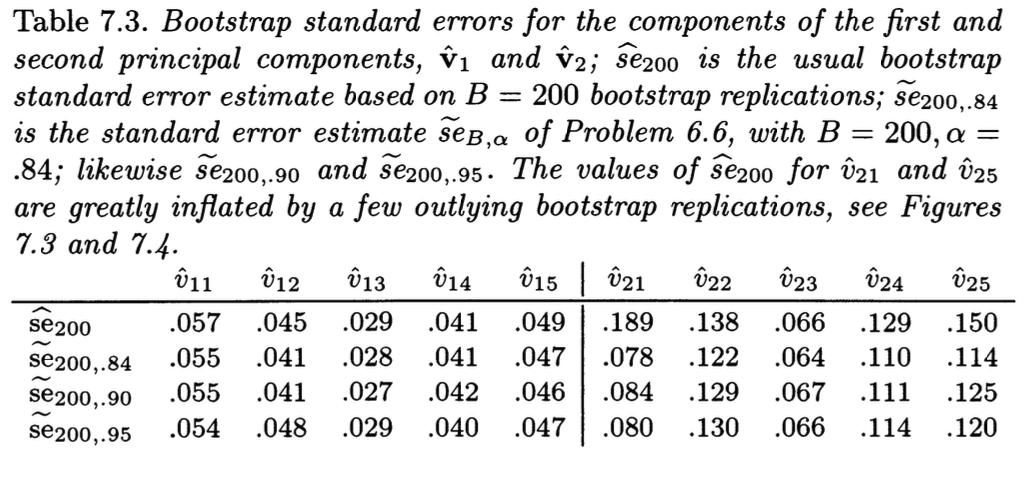
\includegraphics[width=0.9\linewidth]{6/t73.png}
\newline
\setcounter{table}{3}
Это не так для $\hbv_2$, в особенности для первой и пятой координаты. На рисунке 7.3 можно увидеть, в чём проблема. На рисунке показаны эмпирические распределения для 200 бутстреп репликаций $\hat v_{ik}^*$, в отдельности для каждого из $i = 1,2,\, k = 1,2,\ldots, 5$. Эмпирические распределения отражены ящиками с усами. Отрезок в центре ящика --- медиана распределения; нижняя и верхняя сторона ящика есть есть соответственно 25-я и 75-я персентиль распределения; усы покрывают всё распределение за исключением некоторых выбросов (определённых по некоторому критерию), которые отмечены звёздочкой.
\\~\\
\noindent
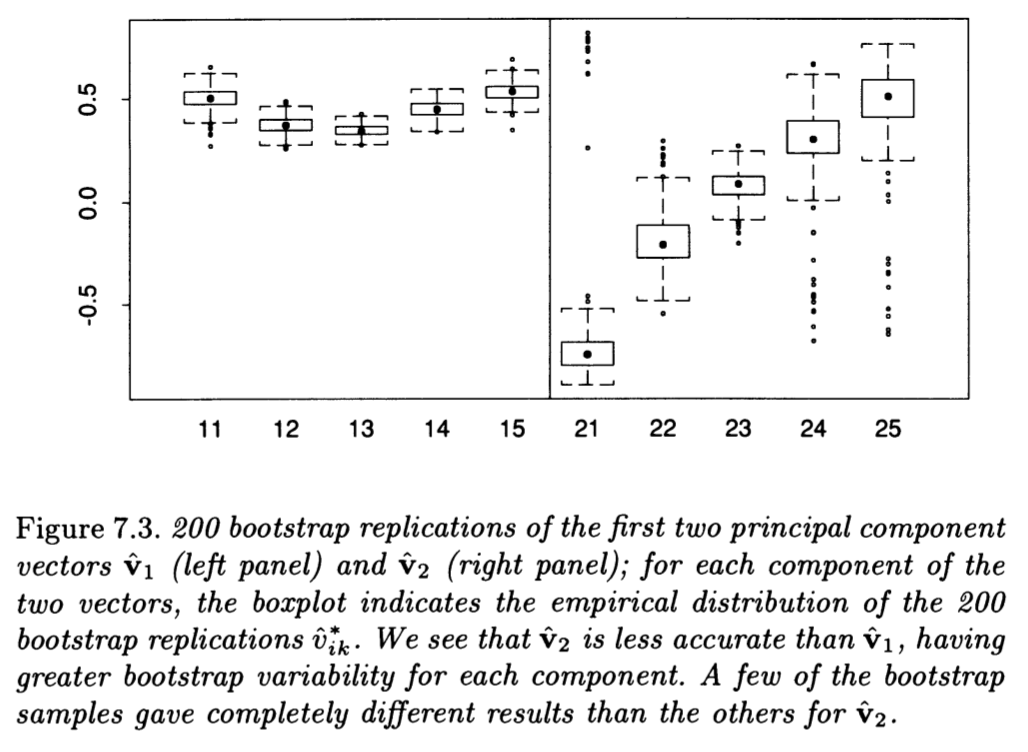
\includegraphics[width=0.9\linewidth]{6/f73.png}
\newline
\setcounter{figure}{3}

Можно увидеть, что большие значения $\seh_{200}$ для $\hat v_{21}$ и $\hat v_{25}$ вызваны несколькими выделяющимися значениями $\hat v_{ik}^*$. Приближённый доверительный интервал $\theta \in \thetahat \pm z^{1-\alpha} \seh$ будет более точным, если выбрать $\sew_{200, \alpha}$ в качестве оценки $\seh$, как минимум для умеренных значений $\alpha$ таких, как $0.843$. Гистограмма значений  $v^*_{21}$ имеет форму нормального распределения со средним в точке $-0.74$ и стандартным отклонением $0.075,$ с небольшим числом точек далеко от гистограммы. Это показатель того, что с малой вероятностью, порядка $1\%$ или $2\%$, что $\hat v_{21}$ оказывается совершенно неточной оценкой настоящего значения $v_{21}$. Если же данное событие не произошло, $\hat v_{21}$ вероятно находится в пределе одного или двух $\sew_{200}$ от $v_{21}$.

На рисунке 7.4 показаны графики бутстреп репликаций $$
\hbv_1^*(b)\tx{ и } \hbv_2^*(b),\qquad b=1,2,\ldots, 200,
$$ 
соединяющие компоненты каждого вектора прямыми. Это более наглядный (хоть и менее точный) показатель вариативности $\hbv_2$, чем предложенные ранее в таблице 7.3 и на рисунке 7.3.
Три конкретных репликации, отмеченные числами 1, 2, и 3, являются выбросами на нескольких компонентах.
\\~\\
\noindent
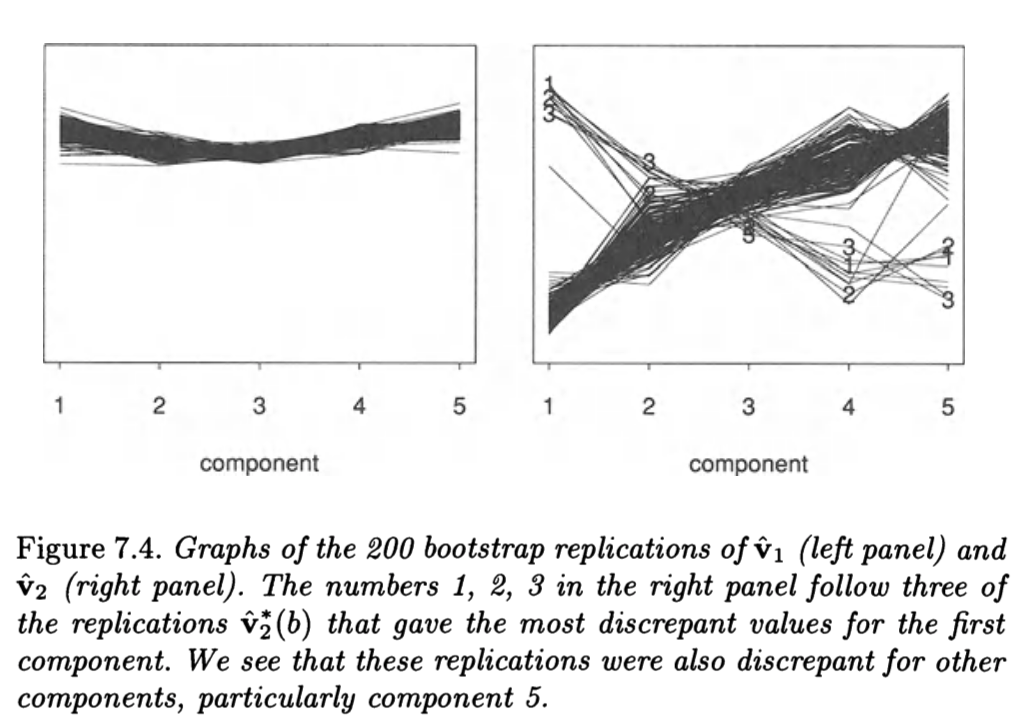
\includegraphics[width=0.9\linewidth]{6/f74.png}
\newline
\setcounter{figure}{4}

Читатель, которому знаком метод главных компонент, может теперь увидеть, что сложности со вторым собственным вектором объясняются проблемой единственности собственных векторов.
Технически, определение собственного вектора $\mathbf v$ также верно и для обратного ему вектора $- \mathbf v$. Алгоритм, который считает собственные числа и собственные значения, может приводить решения с разными знаками у $\hbv_1,\hbv_2,\ldots$ Репликации 1 и 2 привели к матрицам $\X^*$, для которых знак $\hbv_2^*$ получился обратным. Такая неопределённость обычно не важна при определении статистических особенностей оценок (хотя хорошо замечать такую неопределённость на основании результата применения бутстрепа). Если перестать учитывать 1 и 2, как происходит при оценке $\sew_{200,\alpha}$, мы видим, что $\hbv_2$ всё равно менее точна, чем $\hbv_1$.





